\documentclass{article}

\usepackage{arxiv}

\usepackage[utf8]{inputenc} % allow utf-8 input
\usepackage[T1]{fontenc}    % use 8-bit T1 fonts
\usepackage{hyperref}       % hyperlinks
\usepackage{url}            % simple URL typesetting
\usepackage{booktabs}       % professional-quality tables
\usepackage{amsfonts}       % blackboard math symbols
\usepackage{nicefrac}       % compact symbols for 1/2, etc.
\usepackage{microtype}      % microtypography
\usepackage{lipsum}
\usepackage{graphicx}
\usepackage{import}
\usepackage{float}
\graphicspath{ {./images/} }

\usepackage{subcaption}

\title{TP 1.2 - ESTUDIO ECONÓMICO-MATEMÁTICO DE APUESTAS EN LA RULETA}


\author{
    Abud Santiago Elias \\
    Legajo 47015 \\
    \texttt{ sabudvicco@gmail.com} \\
    %% examples of more authors
    \And
    Buchhamer Ariel \\
    Legajo 46217\\
    \texttt{arielbuchhamer1@outlook.com} \\
    \And
    Castellano Marcelo \\
    Legajo 39028 \\
    \texttt{marce.geek22@gmail.com} \\
    \And
    Dolan Guillermo Patricio \\
    Legajo 46101\\
    \texttt{guillermo230899@gmail.com} \\
    \And
    Navarro Franco \\
    Legajo 46387 \\
    \texttt{franconavarro1889@gmail.com} \\
%% \AND
%% Coauthor \\
%% Affiliation \\
%% Address \\
%% \texttt{email} \\
%% \And
%% Coauthor \\
%% Affiliation \\
%% Address \\
%% \texttt{email} \\
%% \And
%% Coauthor \\
%% Affiliation \\
%% Address \\
%% \texttt{email} \\
}

\usepackage[spanish]{babel}
\begin{document}
  \maketitle
  \begin{abstract}
    El juego de la ruleta es un juego de casino muy popular y existen diversas estrategias que presuntamente permitirían vencer las probabilidades y ganar ``dinero fácil'', especialmente populares entre jugadores inexpertos o poco formados en la teoría de probabilidad. Por ello hemos realizado un estudio de simulación para poner a prueba tres estrategias elegidas (martingala, d'Alembert y Fibonacci), bajo los supuestos de capital infinito y capital acotado. Hemos descubierto/nuestros resultados/descubrimientos... % adelanto/esbozo de lo más importante de la conclusión
  \end{abstract}

    \keywords{
    Simulación \and Ruleta \and Apuestas \and Estrategias
    }



% keywords can be removed
%\keywords{First keyword \and Second keyword \and More}


    \section{Introducción}
    La ruleta es un juego de azar típico de los casinos, cuyo nombre viene del término francés roulette,
    que significa ``ruedita'' o ``rueda pequeña''. Su uso como elemento de juego de azar, aún
    en configuraciones distintas de la actual, no está documentado hasta bien entrada la Edad Media.
    Es de suponer que su referencia más antigua es la llamada Rueda de la Fortuna, de la que hay
    noticias a lo largo de toda la historia, prácticamente en todos los campos del saber humano.

    Una ruleta posee un sistema de apuestas denominado ``Martingala'', que es un sistema de apuestas progresivo,
    en el cual se dobla la apuesta tras una pérdida, y se continúa jugando normalmente si se gana.

    Por otro lado, también se tiene el sistema D'Alembert, que es mucho más seguro que el método anterior.
    Este sistema se usa principalmente cuando se apuesta a las apuestas exteriores,
    es decir rojo/negro, par/impar, y 1-18/19-36. La asunción básica de esta estrategia de apuestas en ruleta,
    es que los aciertos en las apuestas exteriores en el largo plazo acabarán balanceándose.
    Así que si hay por ejemplo, una racha de rojos, es algo que solo puede ser temporal.
    Al final, el rojo y el negro acabarán más o menos a la par.

    Otro de los métodos que posee la ruleta, es el sistema Fibonacci, el cual es una de las estrategias
    más famosas y más exitosas entre los jugadores. Este método se basa en la secuencia de Fibonacci,
    una secuencia matemática que es una progresión acumulativa,
    ya que cada siguiente número es igual a la suma de los dos números que lo preceden, y que además,
    es infinita. En dicho sistema, se puede apostar a: rojo/negro, par/impar y números del 1-18/19-36.
    En caso de que la primera apuesta resulta ser ganadora, simplemente se comienza la secuencia de nuevo.
    Distinto es cuando se gana en una apuesta que no es la primera, en lo cual se tiene que retroceder dos pasos.
    Esto sigue hasta que se alcanza el inicio de la secuencia y se obtiene un beneficio.
    Sin embargo, si la racha de partidas perdidas es considerable es necesario volver al inicio y
    empezar de nuevo.








    \section{Descripción del trabajo}
    \label{sec:headings}
    Mediante un programa en Python 3.7 simulamos el comportamiento de una ruleta mediante
    los sistemas de apuestas denominados ``Martingala'', ``D´Alembert'' y ``Fibonacci''.

    Realizadas las tiradas correspondientes, se muestra si el jugador ganó o perdió,
    y se exhibe su capital actual. Además se obtienen los resultados que son reflejados en las gráficas.

    Las tres estrategias responden a los mismos datos generados aleatoriamente y realizan la misma apuesta (rojo o
    negro) para compararlas justamente (que ninguna estrategia tenga corridas más favorables que otra).

    \section{Marco teórico}

    Frecuencia relativa: Magnitud que mide la cantidad de repeticiones que puede tener un suceso por unidad de tiempo.
    \begin{equation}
        f_{i} = f_{r}(x_{i}) = \frac {n_{i}}{N}
    \end{equation}

    Estrategia Martingala: Estrategia de apuestas que consiste en hacer una apuesta inicial y subsiguientemente duplicar la apuesta al perder o regresar a la apuesta inicial al ganar.

    Estrategia d'Alembert: Estrategia de apuestas que consiste en hacer una apuesta inicial y subsiguientemente aumentar la apuesta en una unidad al perder o regresar a la apuesta inicial al ganar.

    Estrategia de Fibonacci: Estrategia de apuestas que consiste en hacer una apuesta inicial y subsiguientemente elevar la apuesta en tantas unidades como tenía la apuesta previa al perder o regresar a la apuesta previa a la anterior al ganar.

\section{Gráficas}
  \subsection{Con capital infinito}
  \subsubsection{Estrategia martingala}
  \begin{figure}[H]
    \centering
    \begin{subfigure}{0.5\textwidth}
      \centering
      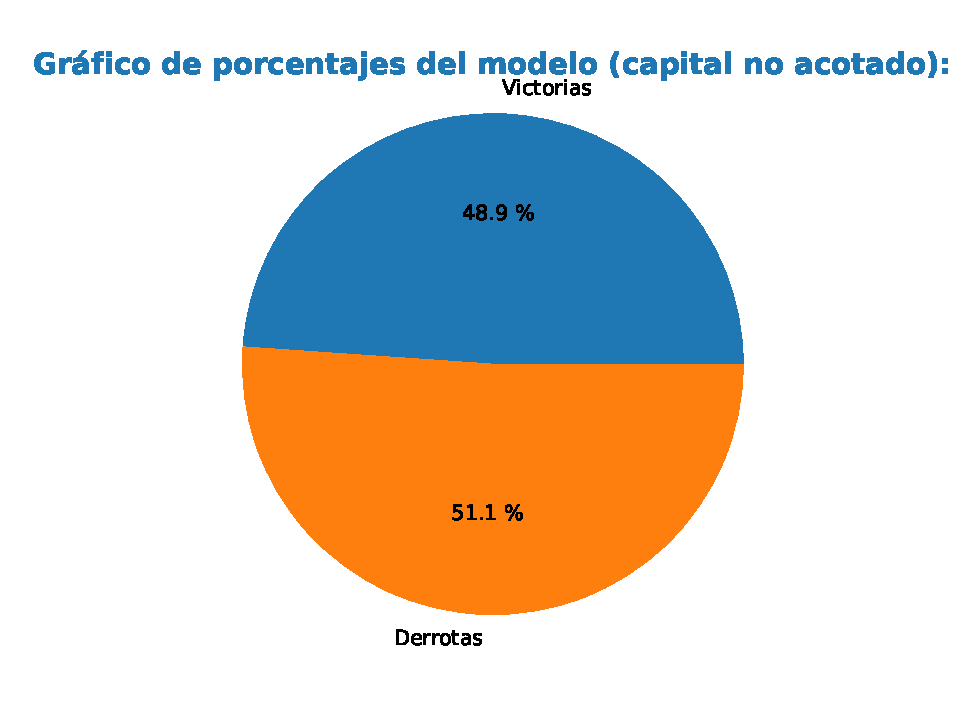
\includegraphics[width=0.8\textwidth]{generated/porcentajes-martingala-no acotado.pdf}
      \caption{Porcentajes de victorias vs. derrotas}
    \end{subfigure}%
	\begin{subfigure}{0.5\textwidth}
	  \centering
      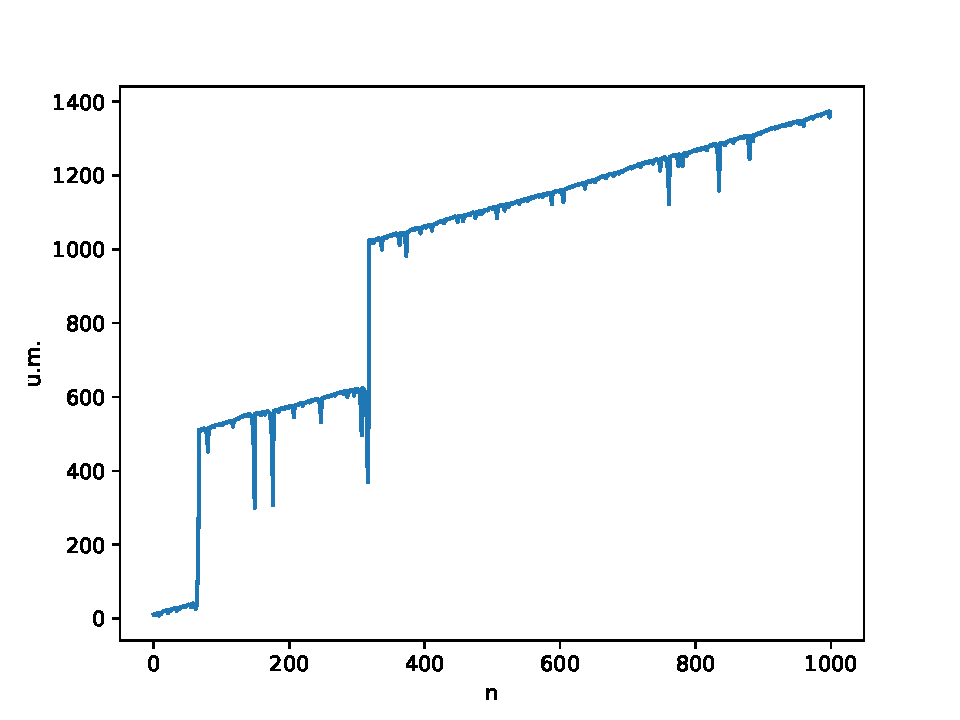
\includegraphics[width=0.8\textwidth]{generated/capital-martingala-no acotado.pdf}
	  \caption{Flujo de caja}
	\end{subfigure}
	\caption{resultados obtenidos aplicando la estrategia martingala en 25 corridas de $n = 1000$ rondas (con capital infinito)}
  \end{figure}

  \subsubsection{Estrategia d’Alembert}
  \begin{figure}[H]
    \centering
    \begin{subfigure}{0.5\textwidth}
      \centering
      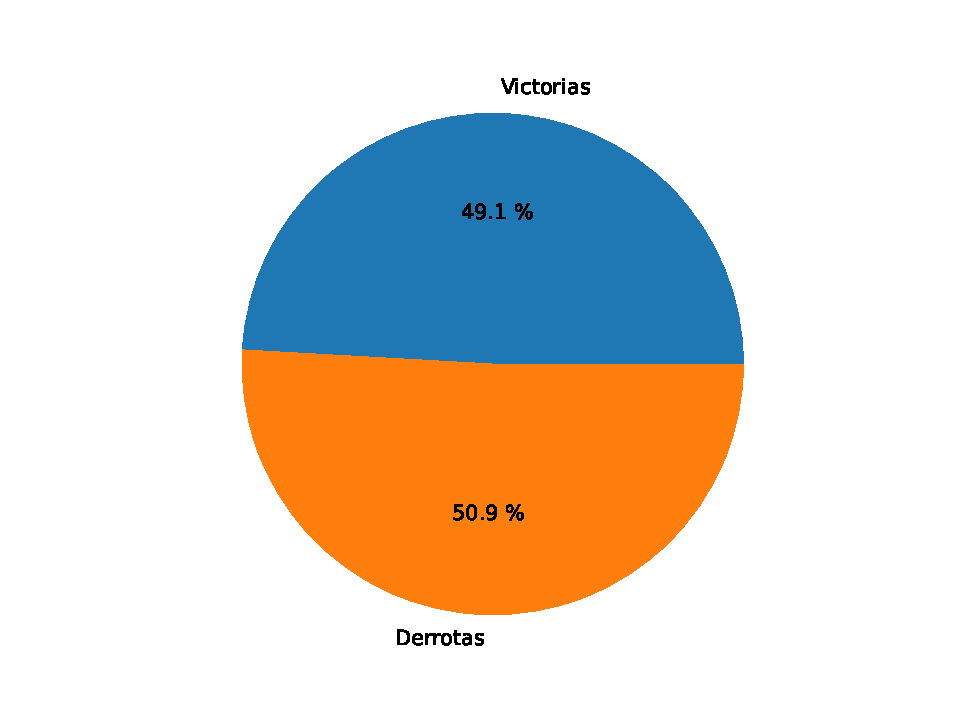
\includegraphics[width=0.8\textwidth]{generated/porcentajes-d'alembert-no acotado.pdf}
      \caption{Porcentajes de victorias vs. derrotas}
    \end{subfigure}%
    \begin{subfigure}{0.5\textwidth}
      \centering
      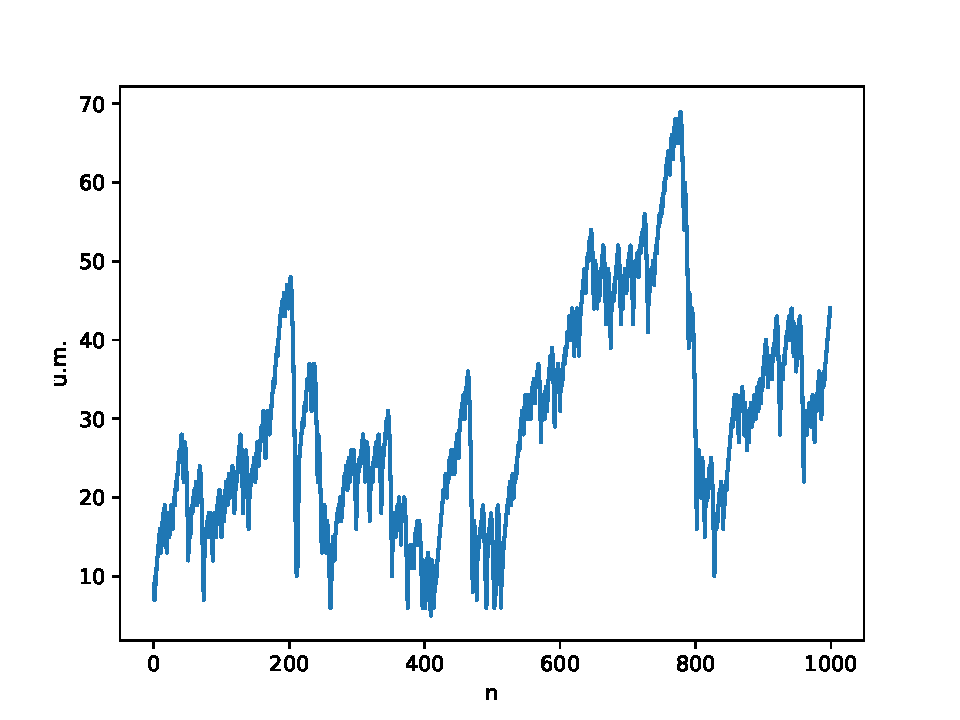
\includegraphics[width=0.8\textwidth]{generated/capital-d'alembert-no acotado.pdf}
      \caption{Flujo de caja}
    \end{subfigure}
    \caption{resultados obtenidos aplicando la estrategia d’Alembert en 25 corridas de $n = 1000$ rondas (con capital infinito)}
  \end{figure}

  \subsubsection{Estrategia Fibonacci}
  \begin{figure}[H]
    \centering
    \begin{subfigure}{0.5\textwidth}
      \centering
      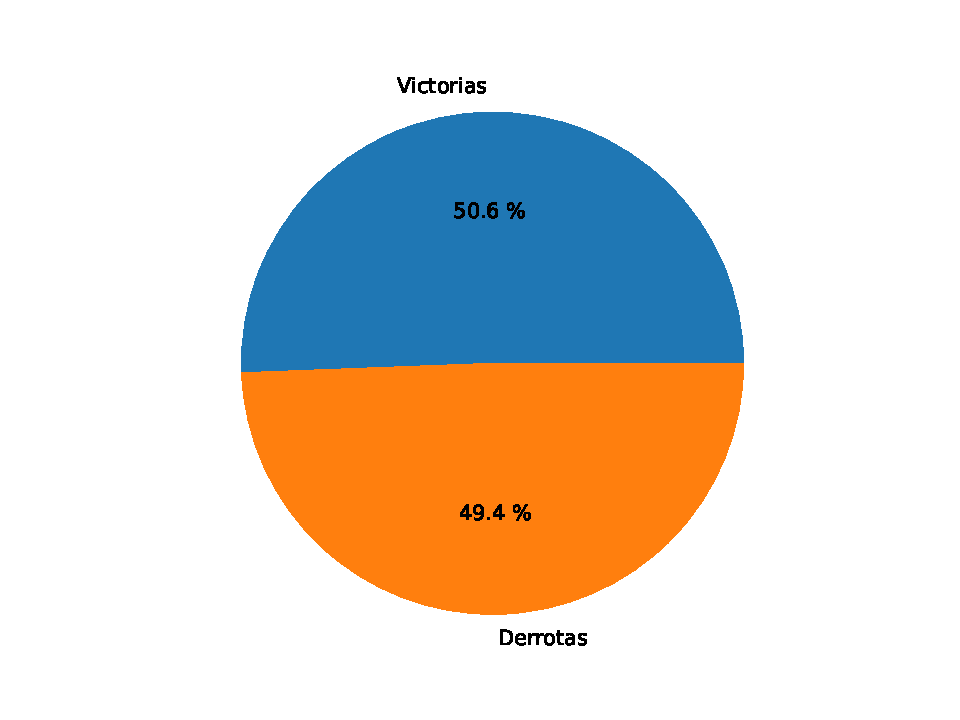
\includegraphics[width=0.8\textwidth]{generated/porcentajes-fibonacci-no acotado.pdf}
      \caption{Porcentajes de victorias vs. derrotas}
    \end{subfigure}%
    \begin{subfigure}{0.5\textwidth}
      \centering
      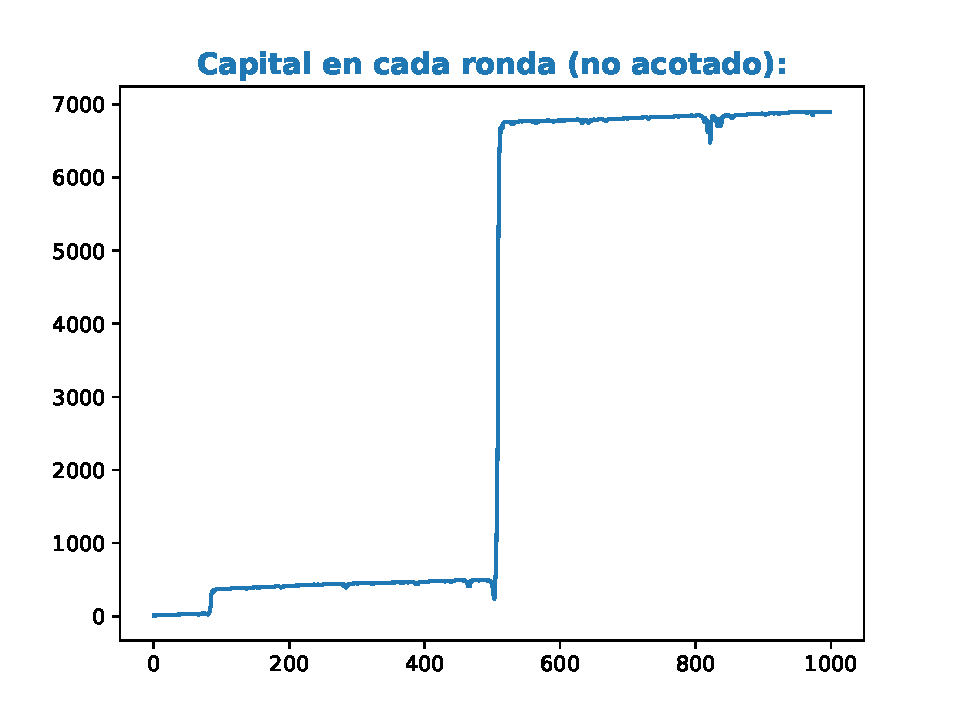
\includegraphics[width=0.8\textwidth]{generated/capital-fibonacci-no acotado.pdf}
      \caption{Flujo de caja}
    \end{subfigure}
    \caption{resultados obtenidos aplicando la estrategia Fibonacci en 25 corridas de $n = 1000$ rondas (con capital infinito)}
  \end{figure}

  \subsubsection{Resumen}

  Vemos que las diferentes estrategias logran resultados muy beneficiosos, pero muy raramente y luego de perder todo el
  capital reiteradas veces.

  \subsection{Con capital acotado}
  \subsubsection{Estrategia martingala}
  \begin{figure}[H]
    \centering
    \begin{subfigure}{0.5\textwidth}
      \centering
      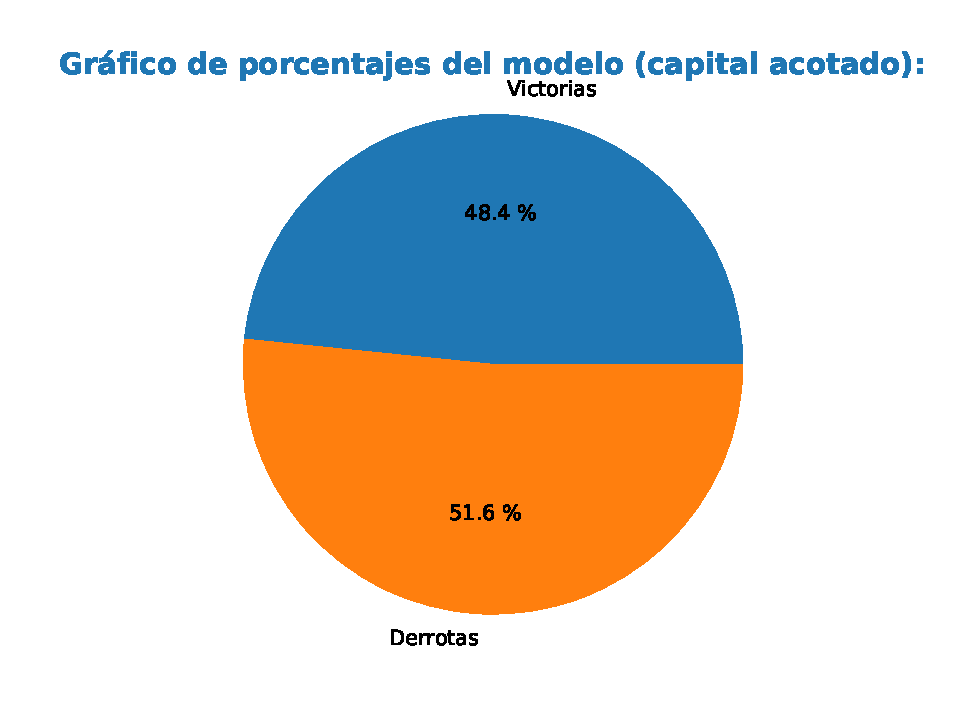
\includegraphics[width=0.8\textwidth]{generated/porcentajes-martingala-acotado.pdf}
      \caption{Porcentajes de victorias vs. derrotas}
    \end{subfigure}%
	\begin{subfigure}{0.5\textwidth}
	  \centering
	    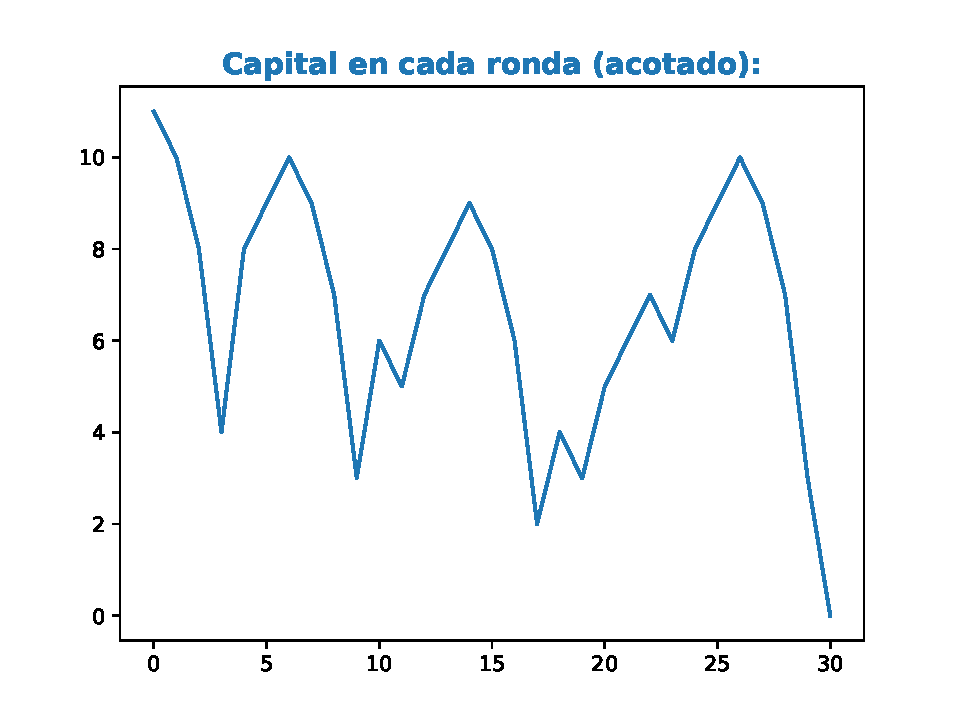
\includegraphics[width=0.8\textwidth]{generated/capital-martingala-acotado.pdf}
      \caption{Flujo de caja}
    \end{subfigure}
    \caption{resultados obtenidos aplicando la estrategia martingala en 25 corridas (con capital acotado)}
  \end{figure}

  \subsubsection{Estrategia d’Alembert}
  \begin{figure}[H]
    \centering
    \begin{subfigure}{0.5\textwidth}
      \centering
      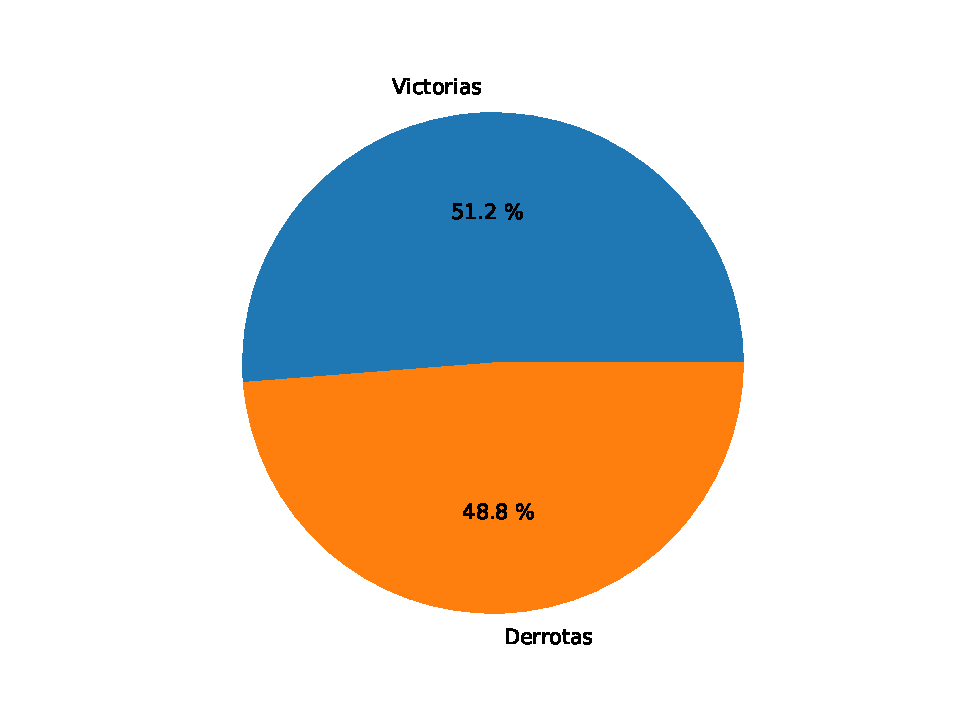
\includegraphics[width=0.8\textwidth]{generated/porcentajes-d'alembert-acotado.pdf}
      \caption{Porcentajes de victorias vs. derrotas}
    \end{subfigure}%
    \begin{subfigure}{0.5\textwidth}
      \centering
      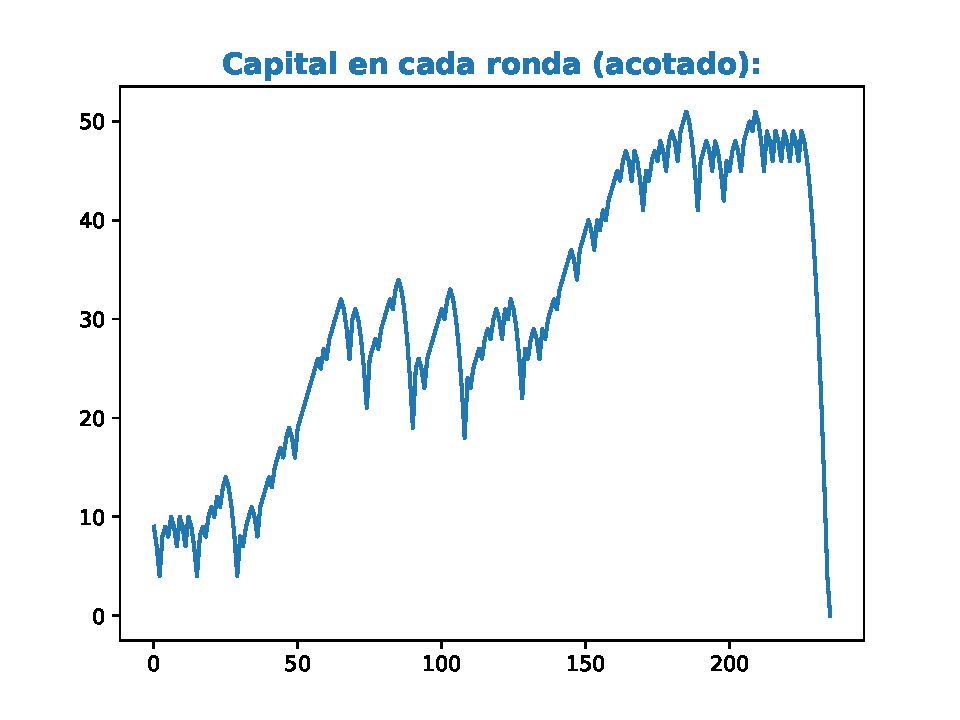
\includegraphics[width=0.8\textwidth]{generated/capital-d'alembert-acotado.pdf}
      \caption{Flujo de caja}
    \end{subfigure}
    \caption{resultados obtenidos aplicando la estrategia d’Alembert en 25 corridas (con capital acotado)}
  \end{figure}

  \subsubsection{Estrategia Fibonacci}
  \begin{figure}[H]
    \centering
    \begin{subfigure}{0.5\textwidth}
      \centering
      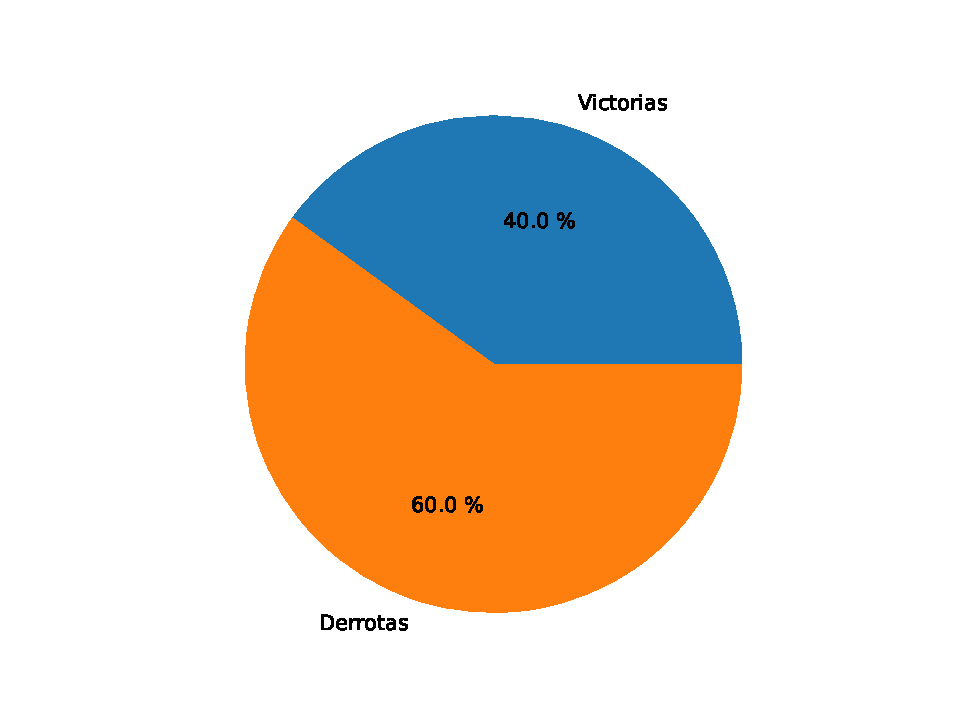
\includegraphics[width=0.8\textwidth]{generated/porcentajes-fibonacci-acotado.pdf}
    \end{subfigure}%
    \begin{subfigure}{0.5\textwidth}
      \centering
      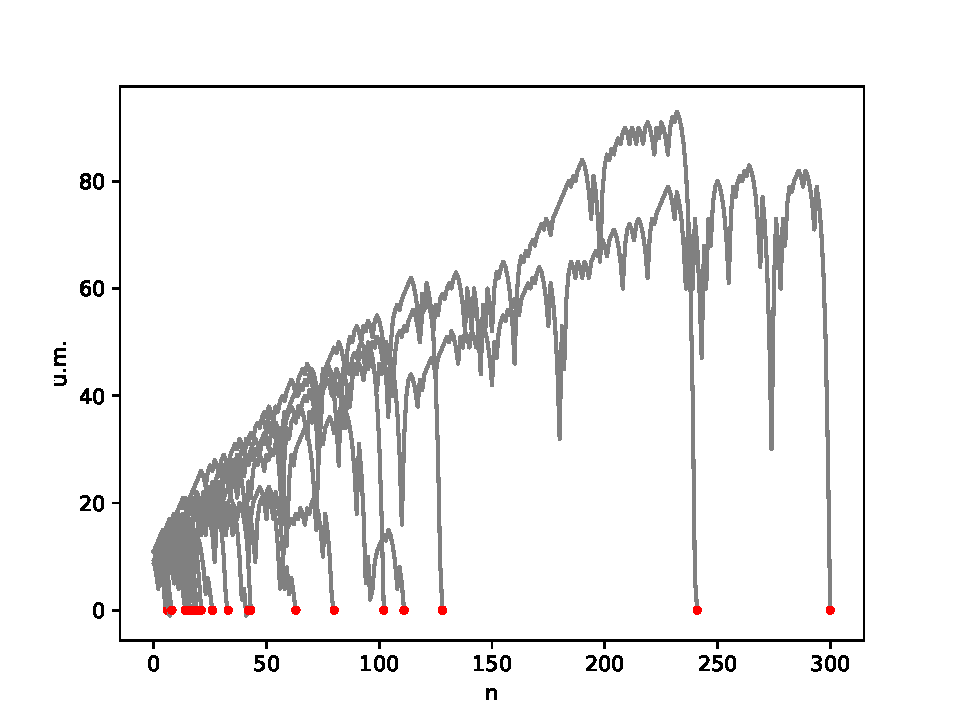
\includegraphics[width=0.8\textwidth]{generated/capital-fibonacci-acotado.pdf}
    \end{subfigure}
    \caption{resultados obtenidos aplicando la estrategia Fibonacci en 25 corridas (con capital acotado)}
  \end{figure}

  \subsubsection{Resumen}

  Si bien en algunos casos se ha llegado a mantener un capital creciente por más de 200 rondas y se han obtenido
  ganancias de más de 60 veces el capital inicial, la verdad es que la mayoría de las rondas no se han extendido a más
  de 40 rondas, y las ganancias de estos casos no han subido a más de 30 veces la apuesta inicial.

  \subsection{Resumen general de las tiradas}
  \begin{figure}[H]
    \centering
    \begin{subfigure}{0.5\textwidth}
      \centering
      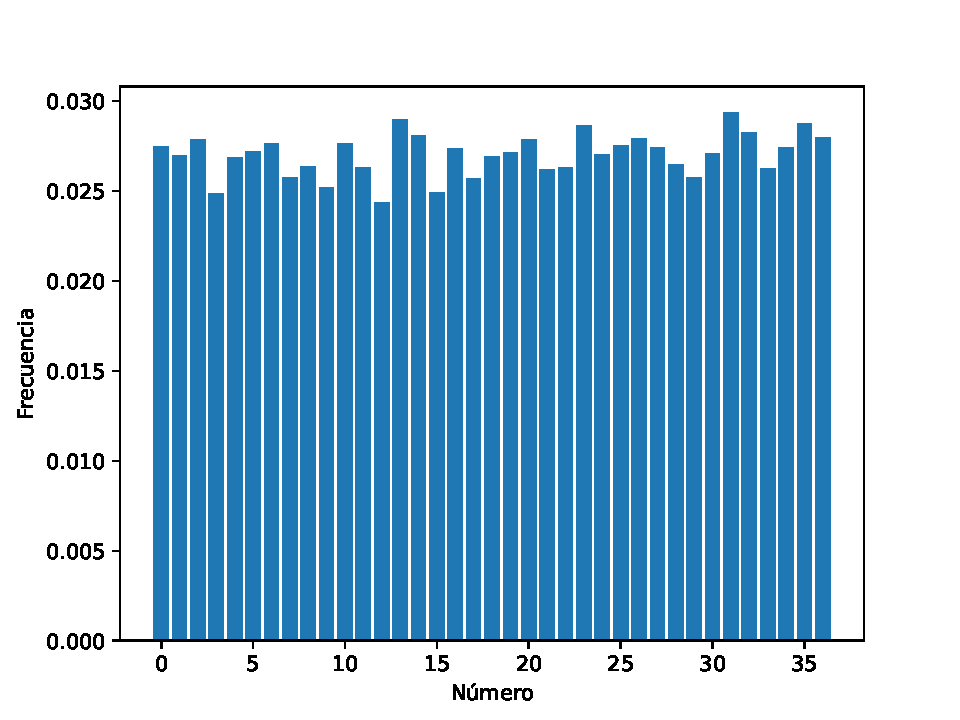
\includegraphics[width=0.8\textwidth]{generated/frec-aparicion.pdf}
      \caption{Frecuencias relativas de aparición por cada número}
    \end{subfigure}%
    \begin{subfigure}{0.5\textwidth}
      \centering
      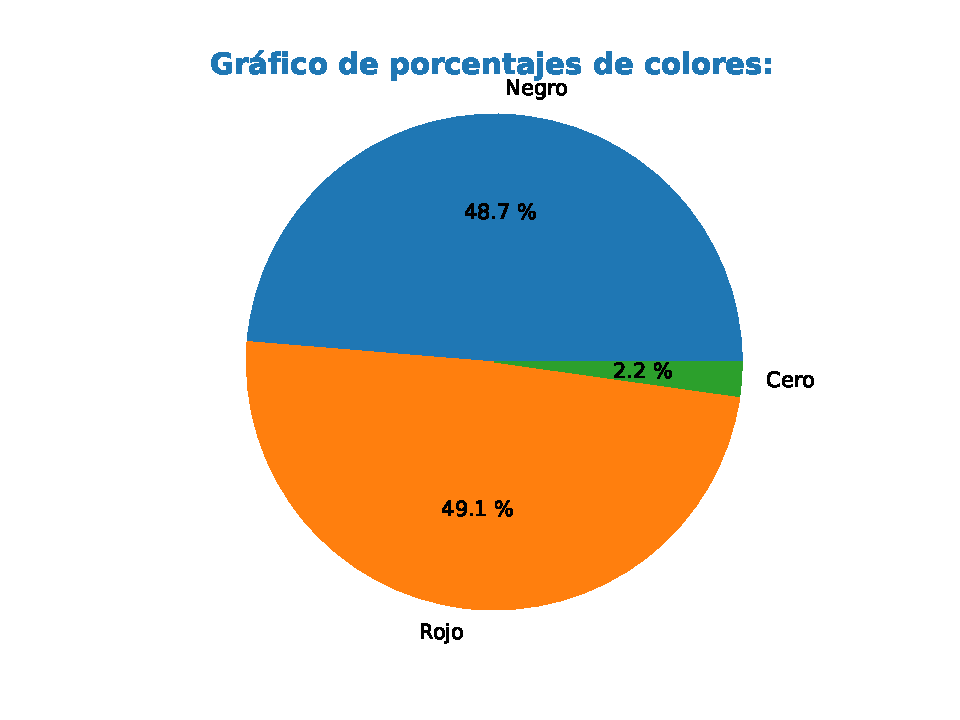
\includegraphics[width=0.8\textwidth]{generated/resumen-colores.pdf}
      \caption{Porcentajes de colores}
    \end{subfigure}
  \end{figure}

\section{Conclusiones}

    Con lo obtenido y trabajado hasta el momento, queda demostrado que estas estrategias no ofrecen resultados
    consistentes y su desempeño es tan azaroso como el juego al que están sujetas.

    Otra observación que se puede hacer es que, aunque no son buenas estrategias a largo plazo, sí ofrecen una gran
    posibilidad de obtener pocas ganancias en un corto plazo, evidenciado por la gran cantidad de veces que las
    estrategias, aún con capital acotado, han sobrevivido y obtenido ganancias tras unas pocas rondas.

\end{document}
